\section{S3 Component - Example}
\label{sec:S3_exmpl}

First example concerns the upload actions of the component.
As shown before, \texttt{part-s3-upload} element calls an \texttt{api-s3-upload} element to handle the transfer from local computer to S3 cloud service.
In the HTML code of \texttt{part-s3-upload} element are implemented both the informations and input tags and the binding with the API.

\subsection{Example One - \texttt{part-s3-upload}}

\begin{lstlisting}[language=html]
<link rel="import"
href="/components/api-s3-upload/api-s3-upload.html">

<dom-module id="part-s3-upload">
  <template>
    <api-s3-upload id="upload"
      file="{{file}}" file-name="{{fileName}}">
    </api-s3-upload>
    <input id="input" type="file" on-change="on_change">
  </template>
</dom-module>

<script>
  Polymer({
    on_change: function () {
      var file = this.$.input.files[0];
      if (!file) {
        return;
      }
      this.fileName = this.fileName || file.name;
      this.file = file;
      this.$.upload.send();
    }
  });
</script>

\end{lstlisting}

In this case, \texttt{api-s3-upload} the is triggered by the \texttt{on-change} function applied on the input box. As shown above \texttt{on-change} function checks the integrity of the file and save its name, then, using \$ selector that puts off to the tag with \texttt{id=``upload''}, triggers the API.

\subsection{Example 2 - \texttt{part-list}}

Second example concerns the retrievement of data to show.
As shown before, \texttt{part-s3-list} element calls an \texttt{api-s3-list} element to handle the GET request and the retrievement of data.
In the HTML code of \texttt{part-s3-list} element there is a binding to \texttt{part-s3-list-item} element that manages the visualization of the retrieved informations.


\begin{lstlisting}[language=html]

<link rel="import"
  href="/components/api-s3-list/api-s3-list.html">
<link rel="import"
  href="part-s3-list-item.html">

<dom-module id="part-s3-list">
  <template>
    <api-s3-list id="list" list="{{list}}">
    </api-s3-list>
    <template is="dom-repeat" items="{{list}}"
      filter="filter">
      <part-s3-list-item item="{{item}}" on-delete="update">
      </part-s3-list-item>
    </template>
  </template>
</dom-module>


<script>
  Polymer({
    update: function () {
      this.$.list.send();
    },
    filter: function (item) {
      var url = 
      'https://' +this.bucket +'.s3.amazonaws.com/'+ item.key;
      item.url = url;
      return item;
    }

  });
</script>

\end{lstlisting}

In this case, \texttt{api-s3-list} the is triggered at page loading time.
Moreover, in \texttt{filter} function, that is called for each object, saves the url for further comunications.

\subsection{Example 3 - \texttt{part-list-item}}

Third example concerns the retrievement and visualization actions of the component.
As shown before, \texttt{part-list-item} is triggered by \texttt{part-list} element. \texttt{part-list-item}, in turn, triggers \texttt{api-s3-delete} API.
This element shows the image saved in S3 Bucket and its additional informations. Moreover \texttt{part-list-item} provides a button to delete the image from the bucket.

\begin{lstlisting}[language=html]
<link rel="import" 
href="/components/api-s3-delete/api-s3-delete.html">
<dom-module id="part-s3-list-item">
  <template>

    <api-s3-delete id="request" file_name="{{item.key}}">
    </api-s3-delete>

    <div id="image">
      <img id="thumb" src="{{item.url}}" 
        preview$="{{preview}}">
      <template is="dom-if" if="{{preview}}">
        <ul id="image_labels">
          <li>Name: 
            <span id="image_details">{{item.key}}</span>
          </li>
          <li>Modified: 
            <span id="image_details">{{item.lastMod}}</span>
          </li>
          <li>Size: 
            <span id="image_details">{{item.size}}</span>
          </li>
        </ul>
        <button id="delete" on-click="on_click">
          Delete
        </button>
      </template>
    </div>

  </template>
</dom-module>
<script>
  Polymer({

    delete_image: function () {
      this.$.request.send();
    }
});
</script>
\end{lstlisting}


In this case, \texttt{api-s3-delete} the is triggered by the \texttt{on-click} function applied on the delete button. As shown above \texttt{on-click} function, using \$ selector that puts off to the tag with \texttt{id=``request''}, triggers the API.


\begin {figure}[h]
\graphicspath{{images/chapter_s3/}}
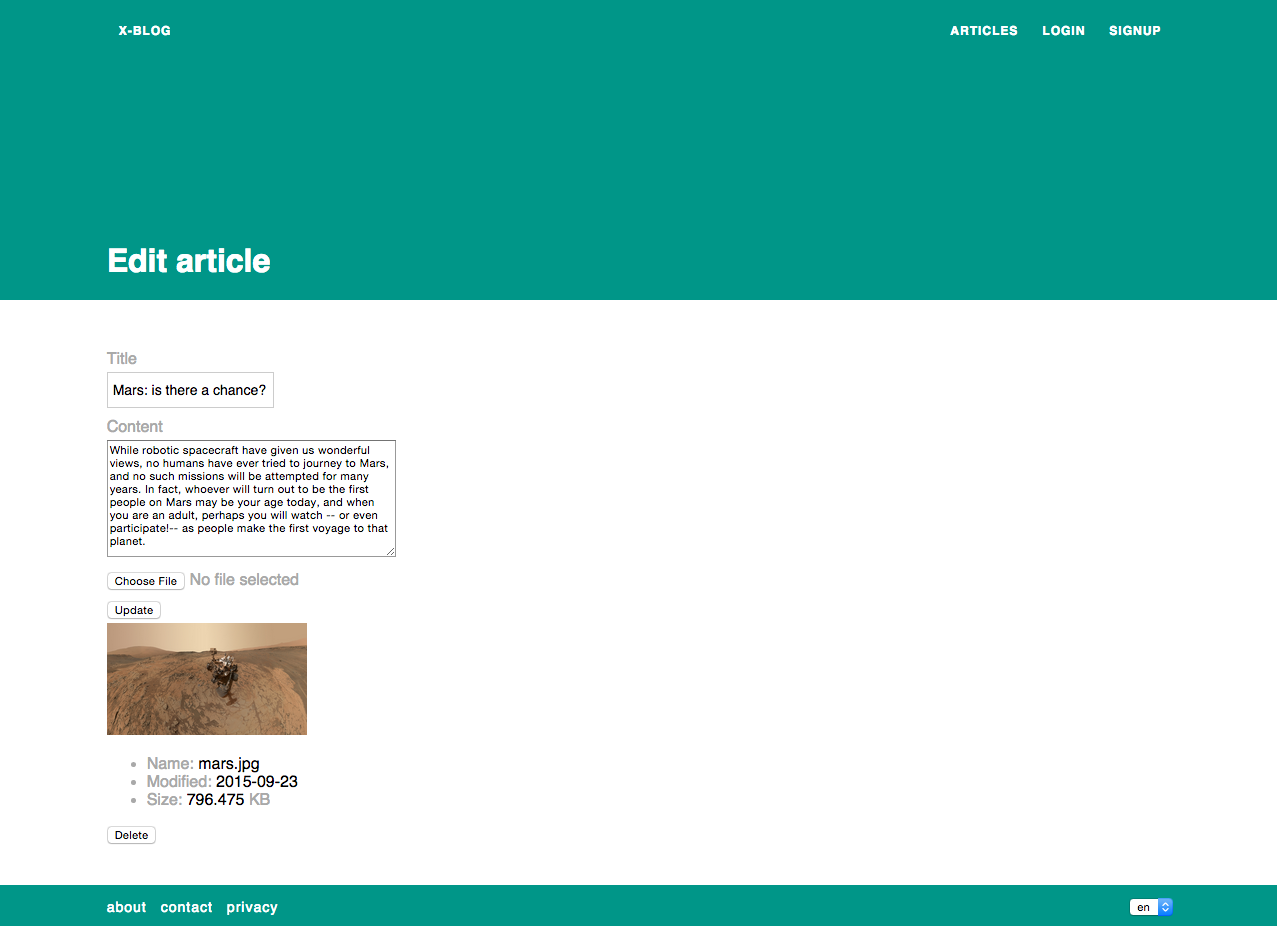
\includegraphics[width=\textwidth]{s3_example}
\caption{S3 Component example - Upload and preview functions}
\end {figure}

